\chapter{Tamanho e poder dos testes, regime e resultados com retorno simples}
\label{app:b2}

Este apêndice complementa os Capítulos~\ref{chap:retornos_linear}
e~\ref{chap:retornos_nao_linear}: traz as simulações de tamanho e poder dos
testes, a regressão com o regime de volatilidade, a correlação entre o erro de
previsão do RBVRP e a inovação do retorno, a comparação da floresta com o
retorno simples e com o log-retorno e, provisoriamente, os resultados da
versão anterior dos Capítulos~\ref{chap:retornos_linear}
e~\ref{chap:retornos_nao_linear}.

% =========================================================
\section{Tamanho e poder dos testes}
\label{sec:apb2-tamanho}

A Tabela~\ref{tab:apb2-tamanho-poder} avalia os testes dos
Capítulos~\ref{chap:retornos_linear} e~\ref{chap:retornos_nao_linear} por
simulação, com as variáveis explicativas reais fixas e $y$ gerado sob a
hipótese nula (painel A) ou com um sinal de $R^2$ populacional $\rho$
(painel B). A rotação testa a independência entre $y$ e as variáveis
explicativas, hipótese mais forte que a de coeficientes nulos, e não é exata
quando o regime de volatilidade muda ao longo da amostra, porque $y$ deixa de
ser estacionário sob a rotação circular. O ruído S2, uma rotação sorteada da
própria série de retornos, fica só nos arquivos de saída: suas réplicas não são
independentes, e o tamanho sob S2 não é estimado com a precisão nominal.

\begin{table}[H]
\centering
\footnotesize
\caption{Tamanho e poder dos testes por simulação.}
\label{tab:apb2-tamanho-poder}
\resizebox{\ifdim\width>\linewidth\linewidth\else\width\fi}{!}{%
\begin{tabular}{llrrrrrrrrr}
\toprule
 & & \multicolumn{3}{c}{$h = 1$} & \multicolumn{3}{c}{$h = 30$} & \multicolumn{3}{c}{$h = 60$} \\ \cmidrule(lr){3-5}\cmidrule(lr){6-8}\cmidrule(lr){9-11}
Caso & Ruído & $\chi^2$ & rot. & boot. & $\chi^2$ & rot. & boot. & $\chi^2$ & rot. & boot. \\
\midrule
\multicolumn{11}{l}{\textit{Painel A: tamanho a 5\% ($\rho = 0$), $L = h+1$}} \\
P16-M & S1 & 0{,}076 & 0{,}044 & 0{,}045 & 0{,}308 & 0{,}058 & 0{,}021 & 0{,}344 & 0{,}060 & 0{,}011 \\
P16-M & S3 & 0{,}084 & 0{,}052 & 0{,}041 & 0{,}259 & 0{,}058 & 0{,}016 & 0{,}330 & 0{,}080 & 0{,}015 \\
P16-F & S1 & 0{,}116 & 0{,}054 & 0{,}045 & 0{,}552 & 0{,}069 & 0{,}010 & 0{,}659 & 0{,}085 & 0{,}002 \\
P16-F & S3 & 0{,}095 & 0{,}048 & 0{,}045 & 0{,}485 & 0{,}056 & 0{,}005 & 0{,}633 & 0{,}103 & 0{,}004 \\
FU-R & S1 & 0{,}051 & 0{,}052 & 0{,}067 & 0{,}137 & 0{,}068 & 0{,}075 & 0{,}159 & 0{,}062 & 0{,}082 \\
FU-R & S3 & 0{,}071 & 0{,}060 & 0{,}082 & 0{,}156 & 0{,}056 & 0{,}073 & 0{,}202 & 0{,}073 & 0{,}096 \\
FU-F & S1 & 0{,}049 & 0{,}050 & 0{,}067 & -- & -- & -- & 0{,}204 & 0{,}058 & 0{,}122 \\
FU-F & S3 & 0{,}074 & 0{,}071 & 0{,}098 & -- & -- & -- & 0{,}193 & 0{,}065 & 0{,}113 \\
\midrule
\multicolumn{11}{l}{\textit{Painel B: poder a 5\% em $h = 30$, ruído S1}} \\
Caso & Teste & $\rho = 0{,}5\%$ & 1\% & 2\% & 5\% & & & & & \\
P16-M & $\chi^2$ aj. & -- & 0{,}102 & 0{,}200 & 0{,}498 & & & & & \\
P16-M & rot. & -- & 0{,}114 & 0{,}230 & 0{,}506 & & & & & \\
P16-M & boot. & -- & 0{,}054 & 0{,}084 & 0{,}304 & & & & & \\
P16-F & $\chi^2$ aj. & -- & 0{,}066 & 0{,}128 & 0{,}254 & & & & & \\
P16-F & rot. & -- & 0{,}086 & 0{,}168 & 0{,}304 & & & & & \\
P16-F & boot. & -- & 0{,}028 & 0{,}032 & 0{,}064 & & & & & \\
FU-R & $\chi^2$ aj. & 0{,}052 & 0{,}108 & 0{,}192 & 0{,}310 & & & & & \\
FU-R & rot. & 0{,}066 & 0{,}120 & 0{,}186 & 0{,}316 & & & & & \\
FU-R & boot. & 0{,}094 & 0{,}152 & 0{,}236 & 0{,}330 & & & & & \\
\bottomrule
\end{tabular}}
\par\smallskip
\parbox{0.95\linewidth}{\footnotesize\textit{Nota}: Casos: P16-M, 16 previsores na amostra de modelagem (1.776 datas); P16-F, 16 previsores nas 987 datas fora da amostra; FU-R e FU-F, fator único com o $\widehat{\text{BVRP}}$ do Ridge e da floresta. rot.: rotação; boot.: bootstrap; $\chi^2$ aj.: $\chi^2$ com o valor crítico ajustado ao tamanho. Simulação com as variáveis explicativas reais fixas e $y$ = constante + ruído (painel A) ou + sinal com $R^2$ populacional $\rho$ (painel B). Ruído: soma de $h$ log-retornos diários reais, S1 sorteados com reposição, S3 em blocos circulares de $\max(60, 2h)$ dias. 1.000 réplicas com $\rho = 0$ e 500 com $\rho > 0$. Testes como nas Tabelas~\ref{tab:retlin-wald-direto} e~\ref{tab:retlin-um-fator}; o bootstrap usa 199 reamostragens. Poder do $\chi^2$ ajustado ao tamanho: valor crítico igual ao quantil de 95\% de $W$ com $\rho = 0$. Em $h = 30$, o $\widehat{\text{BVRP}}$ da floresta não foi simulado (--). O ruído S2 (rotação sorteada da série real) fica só nos arquivos de saída: suas réplicas são rotações da mesma série e não são independentes, de modo que o tamanho sob S2 não é estimado com a precisão nominal. O poder foi simulado só com o ruído S1; o S3 entra só com $\rho = 0$. Os ruídos não reproduzem a dependência de Stambaugh, entre a inovação do retorno e as inovações futuras das variáveis explicativas.}
\end{table}


% =========================================================
\section{Regime de volatilidade}
\label{sec:apb2-regime}

A Tabela~\ref{tab:apb2-regime} estima a regressão do retorno no BVRP previsto
pelo Ridge com inclinações diferentes nos regimes de baixa e de alta
volatilidade, com os cortes fixo e reestimado em cada origem, em $h = 30$ e
$h = 60$. A Seção~\ref{sec:retlin-um-fator} discute os resultados.

\begin{table}[H]
\centering
\footnotesize
\caption{Retorno de $h$ dias, $\widehat{\text{BVRP}}$ do Ridge e regime de volatilidade.}
\label{tab:apb2-regime}
\begin{tabular}{lrrrrr}
\toprule
$H_0$ & gl & $W$ & $p_{\chi^2}$ & $p$ rotação & $p$ bootstrap \\
\midrule
\multicolumn{6}{l}{\textit{Corte fixo, $h = 30$}: $\hat\beta$ = $-$2{,}70, $\hat\delta$ = 4{,}88, $\hat\gamma$ = 2{,}30; 68{,}6\% das datas no regime de alta} \\
$\gamma = 0$ & 1 & 4{,}04 & 0{,}044 & 0{,}101 & 0{,}180 \\
$\delta = \gamma = 0$ & 2 & 4{,}99 & 0{,}083 & 0{,}240 & 0{,}310 \\
$\beta = \delta = \gamma = 0$ & 3 & 8{,}60 & 0{,}035 & 0{,}266 & 0{,}287 \\
\multicolumn{6}{l}{\textit{Corte fixo, $h = 60$}: $\hat\beta$ = $-$4{,}60, $\hat\delta$ = 6{,}13, $\hat\gamma$ = 3{,}43; 68{,}6\% das datas no regime de alta} \\
$\gamma = 0$ & 1 & 4{,}10 & 0{,}043 & 0{,}156 & 0{,}188 \\
$\delta = \gamma = 0$ & 2 & 6{,}86 & 0{,}032 & 0{,}254 & 0{,}233 \\
$\beta = \delta = \gamma = 0$ & 3 & 12{,}44 & 0{,}006 & 0{,}269 & 0{,}242 \\
\multicolumn{6}{l}{\textit{Corte reestimado em cada origem, $h = 30$}: $\hat\beta$ = $-$1{,}88, $\hat\delta$ = 4{,}20, $\hat\gamma$ = 1{,}46; 74{,}9\% das datas no regime de alta} \\
$\gamma = 0$ & 1 & 2{,}30 & 0{,}129 & 0{,}300 & 0{,}314 \\
$\delta = \gamma = 0$ & 2 & 2{,}31 & 0{,}315 & 0{,}689 & 0{,}585 \\
$\beta = \delta = \gamma = 0$ & 3 & 6{,}95 & 0{,}073 & 0{,}447 & 0{,}398 \\
\multicolumn{6}{l}{\textit{Corte reestimado em cada origem, $h = 60$}: $\hat\beta$ = $-$3{,}90, $\hat\delta$ = 4{,}81, $\hat\gamma$ = 2{,}69; 74{,}9\% das datas no regime de alta} \\
$\gamma = 0$ & 1 & 2{,}86 & 0{,}091 & 0{,}237 & 0{,}335 \\
$\delta = \gamma = 0$ & 2 & 3{,}51 & 0{,}173 & 0{,}682 & 0{,}505 \\
$\beta = \delta = \gamma = 0$ & 3 & 11{,}12 & 0{,}011 & 0{,}450 & 0{,}358 \\
\bottomrule
\end{tabular}
\par\smallskip
\parbox{0.95\linewidth}{\footnotesize\textit{Nota}: $R^{\log}_{t,h} = a + \beta\,\widehat{\text{BVRP}}_t + \delta D_t + \gamma D_t\,\widehat{\text{BVRP}}_t + \varepsilon_{t+h}$, com o $\widehat{\text{BVRP}}$ do Ridge, nas 987 datas fora da amostra. $D_t = 1$ se $\text{VH}_{t-29:t}$ supera o corte de $37{,}3\%$ a.a. (fixo) ou o corte vigente na origem (reestimado). $W$ com HAC de $h+1$ defasagens. Rotação de Freedman--Lane: o resíduo do modelo restrito, sem as colunas da hipótese, é deslocado circularmente e somado ao ajustado restrito; em $\beta = \delta = \gamma = 0$ equivale à rotação de $y$. $g_h = \max(90, 3h)$. Bootstrap de pares em blocos circulares de $\max(30, 2h)$ dias, 1.999 reamostragens, centrado em $\hat\beta$. O $\widehat{\text{BVRP}}$ é tratado como dado.}
\end{table}


% =========================================================
\section{Correlação entre o erro de previsão e a inovação do retorno}
\label{sec:apb2-corr-e-u}

O RBVRP de $t$ e o retorno de $t$ a $t+30$ usam os mesmos retornos diários.
Se o erro de previsão do RBVRP se correlacionasse com a inovação do retorno, a
regressão do retorno no BVRP previsto teria um viés adicional. A
Tabela~\ref{tab:apb2-corr-e-u} mede essa correlação nas 987 datas fora da
amostra.

\begin{table}[H]
\centering
\footnotesize
\caption{Correlação entre o erro de previsão do RBVRP e a inovação do retorno de 30 dias.}
\label{tab:apb2-corr-e-u}
\setlength{\tabcolsep}{4pt}
\resizebox{\ifdim\width>\linewidth\linewidth\else\width\fi}{!}{%
\begin{tabular}{lrrrccc}
\toprule
Modelo & corr & EP HAC & $p$ HAC & IC 95\% HAC & IC 95\% boot. & Sem sobrep. \\
\midrule
\multicolumn{7}{l}{\textit{Painel A: inovação A2}} \\
Ridge & $-$0{,}022 & 0{,}194 & 0{,}909 & [$-$0{,}402; 0{,}357] & [$-$0{,}397; 0{,}364] & $-$0{,}008 [$-$0{,}213; 0{,}088] \\
Floresta & $-$0{,}053 & 0{,}195 & 0{,}784 & [$-$0{,}435; 0{,}328] & [$-$0{,}418; 0{,}361] & $-$0{,}046 [$-$0{,}253; 0{,}063] \\
Ridge, $\hat f - \text{IV}$ & $-$0{,}087 & 0{,}172 & 0{,}612 & [$-$0{,}425; 0{,}250] & [$-$0{,}427; 0{,}254] & $-$0{,}085 [$-$0{,}251; 0{,}000] \\
Floresta, $\hat f - \text{IV}$ & $-$0{,}091 & 0{,}174 & 0{,}600 & [$-$0{,}433; 0{,}250] & [$-$0{,}433; 0{,}265] & $-$0{,}099 [$-$0{,}241; 0{,}025] \\
\midrule
\multicolumn{7}{l}{\textit{Painel B: correlação por inovação}} \\
Modelo & A1 & A2 & A3 & A4 & & \\
Ridge & $-$0{,}037 & $-$0{,}022 & $-$0{,}028 & $-$0{,}028 & & \\
Floresta & $-$0{,}089 & $-$0{,}053 & $-$0{,}091 & $-$0{,}092 & & \\
Ridge, $\hat f - \text{IV}$ & $-$0{,}091 & $-$0{,}087 & $-$0{,}113 & $-$0{,}113 & & \\
Floresta, $\hat f - \text{IV}$ & $-$0{,}098 & $-$0{,}091 & $-$0{,}120 & $-$0{,}120 & & \\
MQO & $-$0{,}066 & $-$0{,}038 & $-$0{,}021 & $-$0{,}021 & & \\
LASSO & $-$0{,}037 & $-$0{,}008 & $-$0{,}033 & $-$0{,}033 & & \\
XGBoost & $-$0{,}090 & $-$0{,}046 & $-$0{,}079 & $-$0{,}080 & & \\
Média histórica & $-$0{,}080 & $-$0{,}040 & $-$0{,}075 & $-$0{,}075 & & \\
HBVRP & $-$0{,}072 & $-$0{,}044 & $-$0{,}082 & $-$0{,}083 & & \\
RBVRP defasado & $-$0{,}067 & $-$0{,}038 & $-$0{,}054 & $-$0{,}056 & & \\
\bottomrule
\end{tabular}}
\par\smallskip
\parbox{0.95\linewidth}{\footnotesize\textit{Nota}: $\hat f - \text{IV}$: forma $\hat f(X_t) - \text{IV}_t$; boot.: bootstrap; sem sobrep.: sem sobreposição. $e_t = \text{RBVRP}_t - \widehat{\text{BVRP}}_t$, o erro de previsão do RBVRP de cada modelo, e $u_t$ a inovação de $R^{\log}_{t,30}$, nas 987 datas fora da amostra. A2 (principal): resíduo do MQO de $R^{\log}_{t,30}$ nas 16 variáveis explicativas; A1: resíduo da regressão de $R^{\log}_{t,30}$ na própria previsão; A3: $R^{\log}_{t,30}$ menos a média histórica fora da amostra; A4: $R^{\log}_{t,30}$ menos a previsão do Ridge direto fora da amostra. EP HAC com 31 defasagens; IC HAC $=$ corr $\pm 1{,}96$ EP. IC bootstrap: percentis de 9.999 reamostragens em blocos circulares de 60 dias, com $u$ fixo. Sem sobreposição: mediana [mínimo; máximo] da correlação nas 30 subamostras de uma data a cada 30 dias. Média histórica, HBVRP e RBVRP defasado são os modelos de referência do Capítulo~\ref{chap:previsao_bvrp}.}
\end{table}


% =========================================================
\section{Ponte com o retorno simples}
\label{sec:apb2-ponte}

A versão anterior do Capítulo~\ref{chap:retornos_nao_linear} aplicava a
floresta ao retorno simples de $h$ dias. A
Tabela~\ref{tab:apb2-ponte-retorno} compara as duas versões, com o mesmo
protocolo e só o alvo trocado. Em $h = 60$, o valor-$p$ de 0,014 do
Diebold--Mariano com o retorno simples não indicava previsibilidade: a
floresta errava mais que a média histórica, com $R^2_{\text{fora}}$ de
$-0{,}358$. A perda se espalha por 168 datas, e não por poucas observações
isoladas: são elas que respondem por metade da soma dos erros quadráticos da
floresta, entre as 987, e nas maiores altas de 60 dias, de 63\% a 75\% em
janeiro de 2024, a floresta erra menos que a média. Com o retorno realizado
winsorizado a 1\% e 99\%, o resultado não muda ($R^2_{\text{fora}}$ de
$-0{,}362$; $p = 0{,}014$). A diferença vem do alvo, por meio dos
hiperparâmetros escolhidos pela validação cruzada. Com o retorno simples,
mais assimétrico, a validação cruzada escolhe em $h = 60$ árvores mais
profundas, sem limite de profundidade em 7 das 33 origens, contra nenhuma com
o log-retorno, e o $R^2$ dentro da amostra, em média nas 33 origens, chega a
0,39, contra 0,18. A previsão da floresta treinada no log-retorno, convertida
por $\exp(\cdot) - 1$, tem $R^2_{\text{fora}}$ de $-0{,}113$ contra a média
histórica do retorno simples e $p = 0{,}19$ no Diebold--Mariano, perto do
resultado com o log-retorno ($-0{,}110$; $p = 0{,}40$).

\begin{table}[H]
\centering
\footnotesize
\caption{Floresta direto no retorno e fator único do Ridge: retorno simples e log-retorno.}
\label{tab:apb2-ponte-retorno}
\begin{tabular}{rrrrrrr}
\toprule
 & \multicolumn{3}{c}{Retorno simples} & \multicolumn{3}{c}{Log-retorno} \\ \cmidrule(lr){2-4}\cmidrule(lr){5-7}
$h$ & $R^2_{\text{fora}}$ & $p$ CW & $p$ DM & $R^2_{\text{fora}}$ & $p$ CW & $p$ DM \\
\midrule
\multicolumn{7}{l}{\textit{Painel A: floresta treinada em cada retorno, contra a média histórica do mesmo retorno}} \\
1 & 0{,}0008 & 0{,}133 & 0{,}850 & 0{,}0000 & 0{,}183 & 0{,}992 \\
5 & $-$0{,}0006 & 0{,}186 & 0{,}964 & 0{,}0050 & 0{,}116 & 0{,}757 \\
10 & 0{,}0001 & 0{,}196 & 0{,}997 & 0{,}0103 & 0{,}122 & 0{,}747 \\
20 & 0{,}0207 & 0{,}108 & 0{,}758 & 0{,}0355 & 0{,}050 & 0{,}587 \\
30 & $-$0{,}0754 & 0{,}197 & 0{,}549 & $-$0{,}0290 & 0{,}103 & 0{,}813 \\
60 & $-$0{,}3580 & 0{,}935 & 0{,}014 & $-$0{,}1097 & 0{,}443 & 0{,}399 \\
\midrule
\multicolumn{7}{l}{\textit{Painel B: $h = 60$, avaliação no retorno simples}} \\
\multicolumn{4}{l}{Previsão $\times$ referência} & $R^2_{\text{fora}}$ & $p$ CW & $p$ DM \\
\multicolumn{4}{l}{Floresta no retorno simples $\times$ média do simples} & $-$0{,}358 & 0{,}935 & 0{,}014 \\
\multicolumn{4}{l}{$\exp(\text{previsão log}) - 1$ $\times$ média do simples} & $-$0{,}113 & 0{,}704 & 0{,}191 \\
\multicolumn{4}{l}{$\exp(\text{previsão log}) - 1$ $\times$ $\exp(\text{média do log}) - 1$} & $-$0{,}056 & 0{,}304 & 0{,}642 \\
\multicolumn{4}{l}{Floresta no log-retorno $\times$ média do log (painel A)} & $-$0{,}110 & 0{,}443 & 0{,}399 \\
\midrule
\multicolumn{7}{l}{\textit{Painel C: fator único do Ridge, $\widehat{\text{BVRP}}$ como regressor}} \\
$h$ & \multicolumn{1}{c}{$\hat\beta_h$} & \multicolumn{1}{c}{EP HAC} & \multicolumn{1}{c}{$p_{\chi^2}$} & \multicolumn{1}{c}{$p$ rotação} & \multicolumn{1}{c}{$p$ bootstrap} & \multicolumn{1}{c}{$R^2$} \\
\cmidrule(lr){2-7}
\multicolumn{7}{l}{Retorno simples} \\
1 & $-$0{,}045 & 0{,}018 & 0{,}011 & 0{,}005 & 0{,}005 & 0{,}0067 \\
5 & $-$0{,}144 & 0{,}064 & 0{,}025 & 0{,}091 & 0{,}015 & 0{,}0152 \\
10 & $-$0{,}250 & 0{,}114 & 0{,}029 & 0{,}100 & 0{,}049 & 0{,}0220 \\
20 & $-$0{,}459 & 0{,}230 & 0{,}046 & 0{,}163 & 0{,}093 & 0{,}0327 \\
30 & $-$0{,}586 & 0{,}347 & 0{,}091 & 0{,}286 & 0{,}166 & 0{,}0323 \\
60 & $-$1{,}433 & 0{,}654 & 0{,}028 & 0{,}110 & 0{,}087 & 0{,}0794 \\
\multicolumn{7}{l}{Log-retorno} \\
1 & $-$0{,}042 & 0{,}018 & 0{,}016 & 0{,}012 & 0{,}005 & 0{,}0060 \\
5 & $-$0{,}144 & 0{,}065 & 0{,}026 & 0{,}094 & 0{,}029 & 0{,}0153 \\
10 & $-$0{,}254 & 0{,}115 & 0{,}028 & 0{,}100 & 0{,}055 & 0{,}0239 \\
20 & $-$0{,}475 & 0{,}234 & 0{,}042 & 0{,}156 & 0{,}092 & 0{,}0381 \\
30 & $-$0{,}615 & 0{,}350 & 0{,}079 & 0{,}236 & 0{,}157 & 0{,}0402 \\
60 & $-$1{,}426 & 0{,}618 & 0{,}021 & 0{,}084 & 0{,}094 & 0{,}0985 \\
\bottomrule
\end{tabular}
\par\smallskip
\parbox{0.95\linewidth}{\footnotesize\textit{Nota}: Floresta aleatória direto no retorno de $h$ dias, nas 987 datas fora da amostra, com o mesmo protocolo nos dois retornos (17 variáveis, mesma grade, 500 árvores, validação cruzada de cinco dobras com embargo $h$, 33 origens, mesma semente); só o alvo muda. Retorno simples: as previsões da floresta no retorno simples; log-retorno: Tabela~\ref{tab:retnl-oos-floresta}. CW unilateral e DM bilateral contra a média histórica, com HAC de $h+1$ defasagens. Painel B: a previsão do log-retorno convertida para retorno simples. Com o realizado winsorizado a 1\% e 99\% e as previsões inalteradas, o $R^2_{\text{fora}}$ em $h = 60$ fica em $-$0{,}362 ($p$ DM 0{,}014). Em $h = 60$, metade da soma dos erros quadráticos da floresta vem de 168 das 987 datas e 80\%, de 363 no retorno simples (168 e 335 no log-retorno). Maiores retornos simples de 60 dias: 25/01/2024, 74{,}9\%; 14/01/2024, 71{,}1\%; 13/01/2024, 70{,}5\%; 28/01/2024, 68{,}4\%; 24/01/2024, 67{,}7\%. Em $h = 60$, a validação cruzada escolhe árvores de profundidade 1 em 18 das 33 origens com o retorno simples e em 31 com o log-retorno, e árvores sem limite de profundidade em 7 e 0; o $R^2$ dentro da amostra, em média nas 33 origens, é 0{,}390 e 0{,}176. Painel C: $R_{t,h} = \alpha_h + \beta_h\,\widehat{\text{BVRP}}_t + \varepsilon_{t+h}$, com o BVRP previsto pelo Ridge, nas 987 datas, com o retorno simples e com o log-retorno em pontos percentuais; HAC com $h+1$ defasagens, rotação e bootstrap de pares em blocos circulares como na Tabela~\ref{tab:retlin-um-fator}; no log-retorno, os números são os daquela tabela.}
\end{table}


% =========================================================
\section{Resultados originais com retorno simples (provisória)}
\label{sec:apb2-provisoria}

\textit{Nota: resultados da versão anterior, com retorno simples e bootstrap
em dois níveis, mantidos até a reescrita do apêndice do regressor gerado
(D7).} Esta seção reproduz, sem alteração de números, o texto, as tabelas e as
figuras da versão anterior dos Capítulos~\ref{chap:retornos_linear}
e~\ref{chap:retornos_nao_linear}, que regrediam o retorno simples no BVRP
previsto e usavam o bootstrap em blocos em
dois níveis para o regressor gerado.

% =========================================================
\subsection{Inferência com o BVRP previsto}
\label{sec:apb2-antigo-inferencia}

O erro-padrão HAC trata $\widehat{\text{BVRP}}_t$ como se fosse observado,
quando ele é estimado no primeiro estágio \citep{pagan1984}. Por isso, a
inferência principal usa o bootstrap em blocos em dois níveis da
Seção~\ref{sec:met-inferencia} \citep{kunsch1989}, um procedimento não
paramétrico: em cada reamostragem, o bootstrap reestima o modelo de previsão em
cada origem, com um treino reamostrado em blocos dentro da própria janela de
treino, e reestima $\beta_h$ com os pares (previsão, retorno) das 987 datas,
também reamostrados em blocos.\footnote{No principal, o $\alpha$ do
Ridge fica fixo, em cada origem, no valor escolhido no
Capítulo~\ref{chap:previsao_bvrp}. Reescolhê-lo por validação cruzada em
cada treino reamostrado distorce o procedimento: blocos repetidos podem cair
no treino e na validação da mesma dobra, e a validação passa a favorecer
penalidades menores. O resultado com o $\alpha$ reescolhido aparece entre os
testes de robustez (a seguir).} A reestimação do
primeiro estágio acrescenta ruído à previsão e, como em todo problema de erro
nas variáveis, atenua o coeficiente: a média dos $\beta^*$ das reamostragens
fica abaixo de $\hat\beta_h$, em módulo. A razão $\lambda_h$ entre as duas
mede essa atenuação e fica entre 0,59 e 0,70. O $\hat\beta_h$ estimado com o
BVRP previsto é, portanto, uma medida conservadora da relação entre o prêmio
e o retorno futuro.

A atenuação também encolhe a dispersão dos $\beta^*$, e comparar
$\hat\beta_h$, que não é atenuado, com o erro-padrão do bootstrap, que é,
misturaria escalas e daria valores-$p$ pequenos demais. O teste usa, por
isso, a mesma escala nos dois termos: o erro-padrão de $\hat\beta_h$ é o do
bootstrap dividido por $\lambda_h$, e o intervalo de confiança é
$\hat\beta_h \pm 1{,}96$ vezes esse erro-padrão.\footnote{Com blocos de 60
dias, o segundo nível reamostra cerca de 16 blocos, e intervalos por
percentis seriam grosseiros; por isso o intervalo usa o erro-padrão. Nas
junções entre blocos, a ordem temporal deixa de valer, limitação comum aos
bootstraps em blocos.} O erro-padrão corrigido fica entre 1,25 e 1,71 vez o
HAC. Com seis horizontes, o limite de Bonferroni é
$0{,}05/6 \approx 0{,}0083$.

% =========================================================
\subsection{Resultados}
\label{sec:apb2-antigo-resultados}

A Tabela~\ref{tab:retlin-principal} e a Figura~\ref{fig:retlin-betas}
apresentam os resultados. O coeficiente é negativo em todos os horizontes e
cresce em módulo com $h$, de $-0{,}045$ em $h = 1$ a $-1{,}43$ em $h = 60$.
Em $h = 30$, um desvio-padrão da previsão do Ridge (4,5 p.p.) corresponde a
cerca de 2,6 p.p. a menos de retorno em 30 dias. Com o erro-padrão HAC, os
valores-$p$ ficam entre 0,011 e 0,091; com o bootstrap em dois níveis, entre
0,043 ($h = 1$) e 0,30. Só $h = 1$ fica abaixo de 0,05 no bootstrap, e nenhum
horizonte passa pelo limite de Bonferroni, nem com o HAC.

\begin{table}[H]
\centering
\footnotesize
\caption{Retorno futuro sobre o BVRP previsto: estimativas e inferência por horizonte.}
\label{tab:retlin-principal}
\begin{tabular}{rrrrrrrcr}
\toprule
 & & \multicolumn{2}{c}{HAC} & \multicolumn{4}{c}{Bootstrap em dois níveis} & \\ \cmidrule(lr){3-4}\cmidrule(lr){5-8}
$h$ & $\hat\beta_h$ & EP & $p$ & $\lambda$ & EP corrigido & $p$ & IC 95\% & $R^2$ \\
\midrule
1 & $-$0{,}045 & 0{,}018 & 0{,}011 & 0{,}59 & 0{,}022 & 0{,}043 & [$-$0{,}089; $-$0{,}001] & 0{,}007 \\
5 & $-$0{,}144 & 0{,}064 & 0{,}025 & 0{,}68 & 0{,}082 & 0{,}080 & [$-$0{,}306; 0{,}017] & 0{,}015 \\
10 & $-$0{,}250 & 0{,}114 & 0{,}029 & 0{,}64 & 0{,}182 & 0{,}170 & [$-$0{,}606; 0{,}107] & 0{,}022 \\
20 & $-$0{,}459 & 0{,}230 & 0{,}046 & 0{,}63 & 0{,}392 & 0{,}242 & [$-$1{,}228; 0{,}310] & 0{,}033 \\
30 & $-$0{,}586 & 0{,}347 & 0{,}091 & 0{,}67 & 0{,}570 & 0{,}303 & [$-$1{,}703; 0{,}530] & 0{,}032 \\
60 & $-$1{,}433 & 0{,}654 & 0{,}028 & 0{,}70 & 0{,}979 & 0{,}143 & [$-$3{,}352; 0{,}485] & 0{,}079 \\
\bottomrule
\end{tabular}
\par\smallskip
\parbox{0.95\linewidth}{\footnotesize\textit{Nota}: $R_{t+h} = \alpha_h + \beta_h\,\widehat{\text{BVRP}}_t + \varepsilon_{t+h}$, com o BVRP previsto pelo Ridge (janela expansiva); 987 datas, de 21/06/2023 a 03/03/2026. $\hat\beta_h$ e EP em pontos percentuais de retorno por ponto percentual de BVRP previsto. HAC: Newey--West com $h+1$ defasagens, que ignora a estimação do BVRP previsto. Bootstrap: 999 reamostragens em blocos de 60 dias; $\lambda$ é a razão entre a média dos $\beta^*$ e $\hat\beta_h$; EP corrigido $=$ EP do bootstrap$/\lambda$; o valor-$p$ e o IC usam o EP corrigido. Limite de Bonferroni para seis horizontes: $0{,}05/6 \approx 0{,}0083$.}
\end{table}


\IfFileExists{figs/retornos_linear/fig_betas.png}{
\begin{figure}[H]
    \centering
    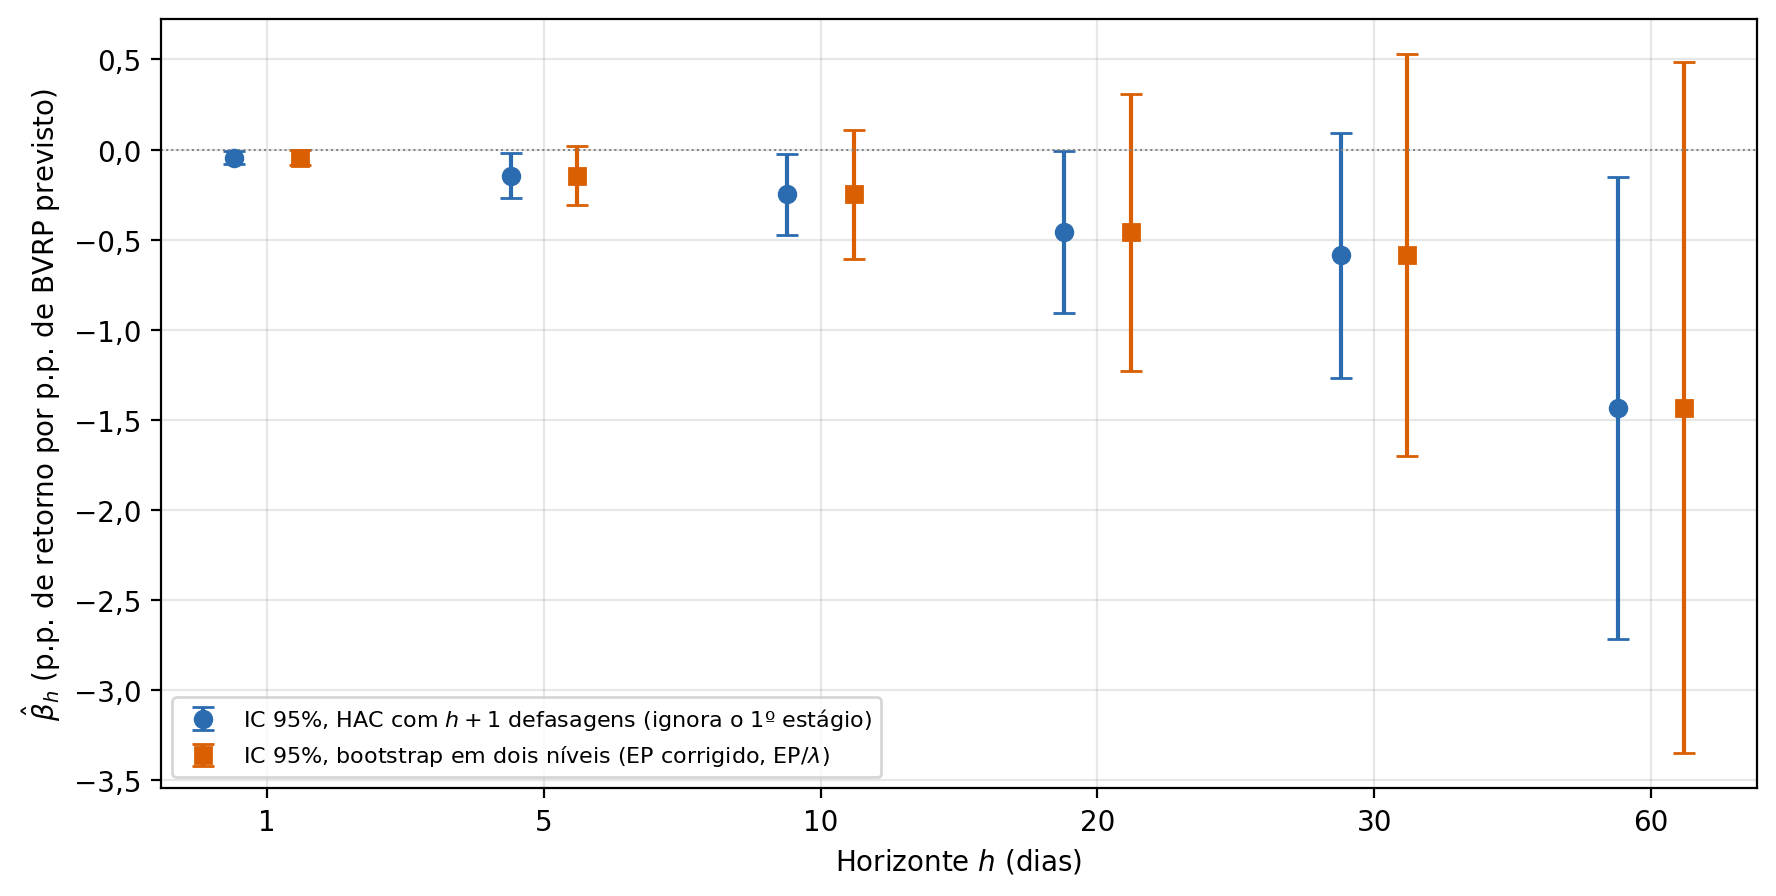
\includegraphics[width=0.9\linewidth]{figs/retornos_linear/fig_betas.png}
    \caption[Coeficiente do retorno futuro sobre o BVRP previsto (Ridge), por horizonte]{Coeficiente do retorno futuro sobre o BVRP previsto (Ridge), por horizonte, com intervalos de confiança de 95\%: erro-padrão HAC com $h+1$ defasagens, que ignora a estimação do BVRP previsto, e bootstrap em dois níveis com o erro-padrão corrigido da atenuação.}
    \label{fig:retlin-betas}
\end{figure}
}{}

Como os seis horizontes são fortemente correlacionados --- os $\beta^*$ de
horizontes vizinhos têm correlação de 0,8 a 0,97 ---, a dissertação testa
também a hipótese conjunta de $\beta_h = 0$ em todos eles
(Tabela~\ref{tab:retlin-conjunto}). O teste de Wald com a covariância dos
$\beta^*$ não rejeita ($p = 0{,}37$), e o resultado se mantém com blocos de 30
e 90 dias ($p = 0{,}21$ e $0{,}27$). O max-$|t|$, um teste de passo único que
toma o maior $|z_h|$ entre os horizontes e tira o valor crítico da
distribuição do máximo nas reamostragens \citep{westfall1993resampling}, em
aplicação com bootstrap em dados dependentes como a de
\citet{romano2005stepwise}, também não rejeita: o menor valor-$p$ ajustado é
0,115, em $h = 1$. Os testes só rejeitam a hipótese conjunta quando ignoram a
estimação do BVRP previsto: com o HAC das seis regressões empilhadas
($p = 0{,}019$) e com o bootstrap só do segundo nível, que mantém as previsões
fixas ($p = 0{,}032$). A diferença entre os dois grupos de testes é o efeito
do regressor gerado.

\begin{table}[H]
\centering
\small
\caption{Teste conjunto nos seis horizontes.}
\label{tab:retlin-conjunto}
\begin{tabular}{lrrr}
\toprule
Inferência & $W$ & $p$ (Wald) & $p$ (max-$|t|$) \\
\midrule
Dois níveis, blocos de 60 dias (principal) & 6{,}46 & 0{,}373 & 0{,}115 \\
Dois níveis, blocos de 30 dias & 8{,}45 & 0{,}207 & 0{,}135 \\
Dois níveis, blocos de 90 dias & 7{,}59 & 0{,}269 & 0{,}149 \\
Dois níveis, $\alpha$ reescolhido & 4{,}08 & 0{,}666 & 0{,}173 \\
Só o 2º nível (ignora o 1º estágio) & 13{,}76 & 0{,}032 & 0{,}022 \\
HAC empilhado, 61 defasagens (ignora o 1º estágio) & 15{,}11 & 0{,}019 & -- \\
\midrule
\multicolumn{4}{l}{\textit{max-$|t|$ por horizonte (principal), valor-$p$ ajustado}} \\
\multicolumn{4}{l}{$h = 1$: 0{,}115; $h = 5$: 0{,}193; $h = 10$: 0{,}345; $h = 20$: 0{,}485; $h = 30$: 0{,}578; $h = 60$: 0{,}290} \\
\bottomrule
\end{tabular}
\par\smallskip
\parbox{0.95\linewidth}{\footnotesize\textit{Nota}: $H_0$: $\beta_h = 0$ nos seis horizontes. Wald: $W = \bar\beta^{*\prime}\,\Sigma^{*-1}\,\bar\beta^*$, com a média e a covariância dos $\beta^*$ do bootstrap, $\chi^2(6)$; equivale ao teste na escala corrigida da atenuação. max-$|t|$: o maior $|z_h|$ entre os horizontes, com valor crítico tirado da distribuição do máximo nas reamostragens (passo único). HAC empilhado: as seis regressões estimadas em conjunto, com Newey--West. Os $\beta^*$ de horizontes vizinhos têm correlação de 0,8 a 0,97, e o número de condição da matriz de correlação é 475.}
\end{table}


A direção do resultado é a mesma de \citet{bollerslev2009expected}. Com
$\text{BVRP}_t = \mathbb{E}(\text{RV}_{t+1:t+30} \mid I_t) - \text{IV}_t$, um
$\beta_h$ negativo equivale a dizer que um prêmio maior, com a IV acima da
volatilidade esperada para os 30 dias seguintes, antecede retornos maiores. A evidência aqui, porém, é fraca: nenhum
horizonte é significante depois das correções.

% =========================================================
\subsection{Testes de robustez}
\label{sec:apb2-antigo-robustez}

A Tabela~\ref{tab:retlin-robustez} reporta os valores-$p$ do bootstrap em
variantes do procedimento. Com blocos de 30 e de 90 dias, os valores-$p$ ficam
entre 0,042 e 0,42; com o $\alpha$ do Ridge reescolhido em cada reamostragem,
entre 0,068 e 0,57. Com a previsão da floresta aleatória, o coeficiente
também é negativo em todos os horizontes e de magnitude parecida, mas nenhum é
significante (valores-$p$ HAC entre 0,15 e 0,61). Só o bootstrap do segundo
nível, que ignora o primeiro estágio, tem um horizonte abaixo do limite de
Bonferroni ($h = 1$, $p = 0{,}003$). O sinal é estável; a significância não
é.

\begin{table}[H]
\centering
\small
\caption{Testes de robustez: valores-$p$ por horizonte.}
\label{tab:retlin-robustez}
\begin{tabular}{lrrrrrr}
\toprule
Variante & $h = 1$ & $h = 5$ & $h = 10$ & $h = 20$ & $h = 30$ & $h = 60$ \\
\midrule
Blocos de 30 dias & 0{,}042 & 0{,}080 & 0{,}130 & 0{,}167 & 0{,}201 & 0{,}060 \\
Blocos de 90 dias & 0{,}050 & 0{,}098 & 0{,}225 & 0{,}326 & 0{,}423 & 0{,}205 \\
$\alpha$ reescolhido & 0{,}068 & 0{,}156 & 0{,}300 & 0{,}442 & 0{,}573 & 0{,}432 \\
Floresta aleatória & 0{,}498 & 0{,}631 & 0{,}783 & 0{,}808 & 0{,}838 & 0{,}700 \\
Só o 2º nível (ignora o 1º estágio) & 0{,}003 & 0{,}022 & 0{,}058 & 0{,}108 & 0{,}178 & 0{,}080 \\
\addlinespace
Floresta aleatória: $\hat\beta_h$ & $-$0{,}057 & $-$0{,}113 & $-$0{,}142 & $-$0{,}294 & $-$0{,}357 & $-$1{,}235 \\
Floresta aleatória: $p$ HAC & 0{,}148 & 0{,}342 & 0{,}487 & 0{,}493 & 0{,}606 & 0{,}333 \\
\bottomrule
\end{tabular}
\par\smallskip
\parbox{0.95\linewidth}{\footnotesize\textit{Nota}: Valores-$p$ do bootstrap em dois níveis na escala corrigida da atenuação (999 reamostragens; 199 na floresta). Principal: Ridge com o $\alpha$ de cada origem fixo e blocos de 60 dias (Tabela~\ref{tab:retlin-principal}). $\alpha$ reescolhido: validação cruzada refeita em cada treino reamostrado. Só o 2º nível: previsões originais fixas, sem correção. Floresta: $\hat\beta_h$ em p.p. por p.p.}
\end{table}


% =========================================================
\subsection{Volatilidade histórica e implícita separadas}
\label{sec:apb2-antigo-componentes}

A equação~\eqref{eq:met-retorno-componentes} substitui o prêmio por seus
componentes observados em $t$, a volatilidade histórica dos 30 dias anteriores
e a IV. Se $\beta_{1,h} + \beta_{2,h} = 0$, a diferença
$\text{VH}_{t-29:t} - \text{IV}_t$, que é o $\text{HBVRP}_t$,
resume o conteúdo das duas medidas. A Tabela~\ref{tab:retlin-componentes}
mostra que os coeficientes têm sinais opostos de $h = 1$ a $h = 20$, a IV com
sinal positivo, e que o teste só rejeita a restrição em $h = 1$ ($p = 0{,}039$;
nos demais horizontes, $p \ge 0{,}18$). Nenhum coeficiente individual é
significante depois da correção de Bonferroni. O teste usa a volatilidade
histórica, a do HBVRP, e não o BVRP previsto: ele diz se a
diferença entre as duas volatilidades observadas em $t$ é uma forma adequada
de combiná-las, não se o prêmio prospectivo prevê o retorno.

\begin{table}[H]
\centering
\small
\caption{Retorno futuro sobre a volatilidade histórica e a implícita.}
\label{tab:retlin-componentes}
\begin{tabular}{rrrrrrr}
\toprule
$h$ & $\hat\beta_{1,h}$ (VH) & $p$ & $\hat\beta_{2,h}$ (IV) & $p$ & $\hat\beta_{1,h} + \hat\beta_{2,h}$ & $p$ \\
\midrule
1 & $-$0{,}009 & 0{,}233 & 0{,}026 & 0{,}023 & 0{,}017 & 0{,}039 \\
5 & $-$0{,}019 & 0{,}493 & 0{,}061 & 0{,}155 & 0{,}042 & 0{,}183 \\
10 & $-$0{,}031 & 0{,}599 & 0{,}090 & 0{,}329 & 0{,}059 & 0{,}329 \\
20 & $-$0{,}025 & 0{,}832 & 0{,}103 & 0{,}564 & 0{,}078 & 0{,}524 \\
30 & 0{,}005 & 0{,}979 & 0{,}074 & 0{,}776 & 0{,}079 & 0{,}667 \\
60 & 0{,}178 & 0{,}514 & 0{,}046 & 0{,}927 & 0{,}224 & 0{,}551 \\
\bottomrule
\end{tabular}
\par\smallskip
\parbox{0.95\linewidth}{\footnotesize\textit{Nota}: $R_{t+h} = \alpha_h + \beta_{1,h}\,\text{VH}_{t-29:t} + \beta_{2,h}\,\text{IV}_t + \varepsilon_{t+h}$, nas mesmas 987 datas; coeficientes em p.p. de retorno por p.p. de volatilidade. Valores-$p$ HAC com $h+1$ defasagens; a última coluna testa $\beta_{1,h} + \beta_{2,h} = 0$.}
\end{table}


% =========================================================
\subsection{Regime de volatilidade}
\label{sec:apb2-antigo-regime}

A equação~\eqref{eq:met-retorno-regime} permite inclinações diferentes nos
regimes de baixa e de alta volatilidade. Com o
corte fixo, a inclinação é mais negativa no regime de baixa, que reúne 31\%
das datas fora da amostra ($-2{,}92$ em $h = 30$, $p = 0{,}005$), e fica perto
de zero no regime de alta ($-0{,}34$; ver Tabela~\ref{tab:retlin-regime}). A
inclinação no regime de baixa passa pelo limite de Bonferroni de $h = 20$ a
$h = 60$, mas a diferença entre os regimes, não: a interação é significante a
5\% de $h = 10$ a $h = 60$, sem passar pelo limite, e o teste conjunto da
variável de regime e da interação só rejeita a 5\% em $h = 60$
($p = 0{,}035$). Com o corte reestimado em cada origem, a diferença deixa de
ser significante (interação com $p \ge 0{,}06$; teste conjunto com
$p \ge 0{,}15$). A diferença entre os regimes é, assim, sugestiva e frágil:
depende da posição do corte, e esses valores-$p$ são do HAC, que ignora a
estimação do BVRP previsto.

\begin{table}[H]
\centering
\small
\caption{Retorno futuro, BVRP previsto e regime de volatilidade.}
\label{tab:retlin-regime}
\begin{tabular}{rrrrrrr}
\toprule
$h$ & Baixa: $\hat\beta_h$ & $p$ & Alta & $\hat\gamma_h$ & $p$ & $p$ (Wald) \\
\midrule
\multicolumn{7}{l}{\textit{Corte fixo} (31{,}4\% das datas no regime de baixa)} \\
1 & $-$0{,}071 & 0{,}155 & $-$0{,}061 & 0{,}011 & 0{,}857 & 0{,}554 \\
5 & $-$0{,}528 & 0{,}034 & $-$0{,}131 & 0{,}396 & 0{,}140 & 0{,}250 \\
10 & $-$1{,}091 & 0{,}015 & $-$0{,}159 & 0{,}932 & 0{,}046 & 0{,}128 \\
20 & $-$2{,}147 & 0{,}006 & $-$0{,}313 & 1{,}834 & 0{,}034 & 0{,}081 \\
30 & $-$2{,}922 & 0{,}005 & $-$0{,}339 & 2{,}583 & 0{,}031 & 0{,}071 \\
60 & $-$5{,}172 & $<$0{,}001 & $-$1{,}034 & 4{,}138 & 0{,}026 & 0{,}035 \\
\addlinespace
\multicolumn{7}{l}{\textit{Corte expansivo} (25{,}1\% das datas no regime de baixa)} \\
1 & $-$0{,}072 & 0{,}227 & $-$0{,}058 & 0{,}014 & 0{,}833 & 0{,}491 \\
5 & $-$0{,}295 & 0{,}176 & $-$0{,}139 & 0{,}156 & 0{,}510 & 0{,}751 \\
10 & $-$0{,}546 & 0{,}145 & $-$0{,}196 & 0{,}350 & 0{,}392 & 0{,}694 \\
20 & $-$1{,}313 & 0{,}055 & $-$0{,}342 & 0{,}971 & 0{,}184 & 0{,}414 \\
30 & $-$2{,}030 & 0{,}037 & $-$0{,}319 & 1{,}711 & 0{,}100 & 0{,}250 \\
60 & $-$4{,}397 & 0{,}005 & $-$1{,}077 & 3{,}319 & 0{,}064 & 0{,}159 \\
\bottomrule
\end{tabular}
\par\smallskip
\parbox{0.95\linewidth}{\footnotesize\textit{Nota}: $R_{t+h} = \alpha_h + \beta_h\,\widehat{\text{BVRP}}_t + \delta_h D_t + \gamma_h D_t\,\widehat{\text{BVRP}}_t + \varepsilon_{t+h}$, com $D_t = 1$ no regime de alta volatilidade. Inclinação no regime de baixa: $\hat\beta_h$; no de alta: $\hat\beta_h + \hat\gamma_h$; em p.p. por p.p. Valores-$p$ HAC com $h+1$ defasagens; Wald: $\delta_h = \gamma_h = 0$. Corte fixo: $37{,}3\%$ a.a., da primeira janela; expansivo: reestimado em cada origem.}
\end{table}


% =========================================================
\subsection{BVRP previsto pela floresta e retorno simples}
\label{sec:apb2-antigo-retnl-resultados}

Os resultados a seguir reproduzem, sem alteração de números, a versão
anterior do Capítulo~\ref{chap:retornos_nao_linear}, cuja forma principal era
o BVRP previsto pela floresta na forma $\hat f(X_t) - \text{IV}_t$
(equação~\eqref{eq:retnl-forma}). Para cada horizonte $h \in \{1, 5, 10, 20, 30, 60\}$, a versão anterior regredia o
retorno simples de $t$ a $t+h$ no BVRP previsto, como na
equação~\eqref{eq:met-retorno-linear}, nas mesmas 987 datas fora da amostra e
com a inferência da Seção~\ref{sec:apb2-antigo-inferencia}: erro-padrão HAC com
$h+1$ defasagens e bootstrap em blocos em dois níveis, que incorpora a
estimação do BVRP previsto. As reamostragens são as mesmas em todos os
horizontes e nos quatro regressores.

A Tabela~\ref{tab:retnl-principal} e a Figura~\ref{fig:retnl-betas}
apresentam os resultados da forma principal. O coeficiente fica entre
$-0{,}076$ e $0{,}070$ p.p. de retorno por p.p. de BVRP previsto, troca de
sinal entre os horizontes, e os valores-$p$ HAC ficam entre 0,55 e 0,94. O
$R^2$ não passa de 0,0014.

\begin{table}[H]
\centering
\small
\caption{Retorno futuro sobre o BVRP previsto pela floresta: estimativas e inferência por horizonte.}
\label{tab:retnl-principal}
\begin{tabular}{rrrrrrr}
\toprule
 & & \multicolumn{3}{c}{HAC} & \multicolumn{2}{c}{Bootstrap em dois níveis} \\ \cmidrule(lr){3-5}\cmidrule(lr){6-7}
$h$ & $\hat\beta_h$ & EP & $p$ & $R^2$ & $\lambda$ & $p$ \\
\midrule
1 & $-$0{,}006 & 0{,}010 & 0{,}553 & 0{,}0003 & 1{,}16 & 0{,}454 \\
5 & $-$0{,}006 & 0{,}038 & 0{,}869 & 0{,}0001 & 1{,}96 & 0{,}757 \\
10 & 0{,}005 & 0{,}066 & 0{,}937 & 0{,}0000 & $-$0{,}35 & -- \\
20 & 0{,}030 & 0{,}136 & 0{,}827 & 0{,}0004 & 0{,}64 & 0{,}904 \\
30 & 0{,}070 & 0{,}209 & 0{,}738 & 0{,}0014 & 0{,}83 & 0{,}801 \\
60 & $-$0{,}076 & 0{,}371 & 0{,}837 & 0{,}0007 & $-$0{,}12 & -- \\
\bottomrule
\end{tabular}
\par\smallskip
\parbox{0.95\linewidth}{\footnotesize\textit{Nota}: $R_{t+h} = \alpha_h + \beta_h\,\widehat{\text{BVRP}}_t + \varepsilon_{t+h}$, com $\widehat{\text{BVRP}}_t = \hat f(X_t) - \text{IV}_t$ e $\hat f$ a floresta aleatória para $\text{VH}_{t+1:t+30}$ (janela expansiva); 987 datas. $\hat\beta_h$ e EP em pontos percentuais de retorno por ponto percentual de BVRP previsto. HAC: Newey--West com $h+1$ defasagens. Bootstrap: 999 reamostragens em blocos de 60 dias; $\lambda$ é a razão entre a média dos $\beta^*$ e $\hat\beta_h$, e o valor-$p$ usa o EP do bootstrap dividido por $\lambda$; com $\lambda \le 0$, a correção não é definida (--).}
\end{table}


\IfFileExists{figs/retornos_nao_linear/fig_betas.png}{
\begin{figure}[H]
    \centering
    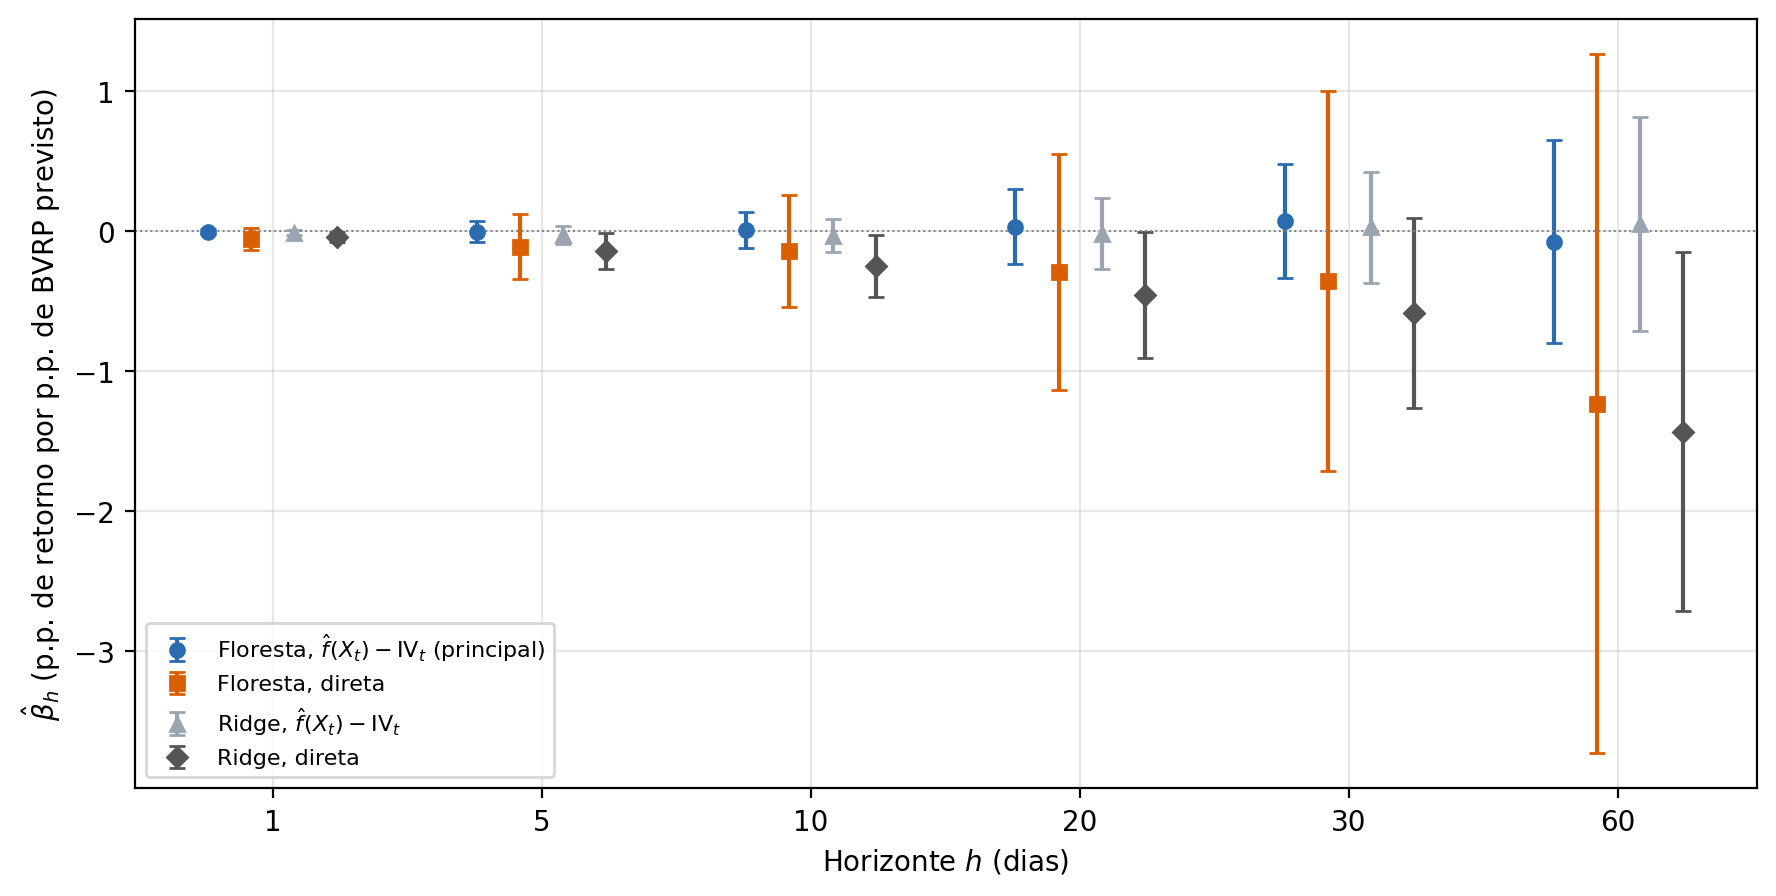
\includegraphics[width=0.9\linewidth]{figs/retornos_nao_linear/fig_betas.png}
    \caption[Coeficiente do retorno futuro sobre o BVRP previsto, por regressor]{Coeficiente do retorno futuro sobre o BVRP previsto, por horizonte e regressor, com intervalos de confiança de 95\% pelo erro-padrão HAC com $h+1$ defasagens.}
    \label{fig:retnl-betas}
\end{figure}
}{}

Com $\hat\beta_h$ perto de zero, a correção de escala do bootstrap deixa de
funcionar. A razão $\lambda_h$ entre a média dos $\beta^*$ e $\hat\beta_h$,
que na Seção~\ref{sec:apb2-antigo-inferencia} mede a atenuação, divide por um
número próximo de zero: fica entre $-2{,}75$ e $3{,}45$ e é negativa em 5 das
18 combinações de horizonte e tamanho de bloco, casos em que o erro-padrão
corrigido não é definido. Nesses casos, a inferência se apoia no erro-padrão
HAC e no teste conjunto, que não usa $\lambda_h$.

O teste conjunto é um teste de significância conjunta de Wald, cuja
estatística dividida pelo número de restrições é a estatística $F$. Ele testa
$\beta_h = 0$ nos seis horizontes com a covariância dos $\beta^*$ do bootstrap
(Tabela~\ref{tab:retnl-conjunto}). Para a forma principal, $\chi^2(6) = 1{,}45$
e $p = 0{,}96$, e o resultado se repete com blocos de 30 e de 90 dias
($p = 0{,}95$ e $0{,}96$), com o max-$|t|$ ($p = 0{,}79$) e com o HAC das seis
regressões empilhadas ($p = 0{,}93$). Ao contrário do Ridge direto, para o qual
os testes que ignoram a estimação do BVRP previsto rejeitam
(Seção~\ref{sec:apb2-antigo-resultados}), nenhum teste rejeita com a floresta,
nas duas formas.

\begin{table}[H]
\centering
\footnotesize
\caption{Teste conjunto nos seis horizontes.}
\label{tab:retnl-conjunto}
\begin{tabular}{lrrrrr}
\toprule
Regressor & $W$ & $p$ (Wald) & $p$ (max-$|t|$) & $p$ (HAC empilhado) & $p$ (só 2º nível) \\
\midrule
Floresta, $\hat f(X_t) - \text{IV}_t$ (principal) & 1{,}45 & 0{,}963 & 0{,}791 & 0{,}925 & 0{,}952 \\
\quad blocos de 30 dias & 1{,}63 & 0{,}950 & 0{,}670 & & \\
\quad blocos de 90 dias & 1{,}48 & 0{,}961 & 0{,}905 & & \\
Floresta, direta & 1{,}12 & 0{,}980 & 0{,}708 & 0{,}234 & 0{,}507 \\
Ridge, $\hat f(X_t) - \text{IV}_t$ & 4{,}39 & 0{,}624 & 0{,}382 & 0{,}233 & 0{,}389 \\
Ridge, direta & 6{,}46 & 0{,}373 & 0{,}115 & 0{,}019 & 0{,}032 \\
\bottomrule
\end{tabular}
\par\smallskip
\parbox{0.95\linewidth}{\footnotesize\textit{Nota}: $H_0$: $\beta_h = 0$ nos seis horizontes. Wald: $W = \bar\beta^{*\prime}\,\Sigma^{*-1}\,\bar\beta^*$, com a média e a covariância dos $\beta^*$ do bootstrap em dois níveis (blocos de 60 dias, salvo indicação), $\chi^2(6)$; continua definido quando $\lambda_h \le 0$. max-$|t|$: valor-$p$ global do maior $|z_h|$. HAC empilhado: as seis regressões em conjunto, Newey--West com 61 defasagens. As duas últimas colunas ignoram a estimação do BVRP previsto.}
\end{table}


% =========================================================
\subsection{Testes de robustez com a floresta}
\label{sec:apb2-antigo-retnl-robustez}

A Tabela~\ref{tab:retnl-robustez} repete a regressão com o BVRP previsto pelos
outros três regressores. Com a floresta na forma direta, o coeficiente é
negativo em todos os horizontes, como na Seção~\ref{sec:apb2-antigo-resultados},
mas nenhum é significante (valores-$p$ HAC entre 0,15 e 0,61). Com o Ridge na
forma $\hat f(X_t) - \text{IV}_t$, os valores-$p$ HAC ficam entre 0,12 e 0,90.
O Ridge direto reproduz a Seção~\ref{sec:apb2-antigo-resultados}. O teste conjunto
não rejeita com nenhum dos três quando a estimação do BVRP previsto é
considerada ($p$ entre 0,37 e 0,98).

\begin{table}[H]
\centering
\small
\caption{Testes de robustez: retorno futuro sobre o BVRP previsto por outros modelos.}
\label{tab:retnl-robustez}
\begin{tabular}{lrrrrrr}
\toprule
 & $h = 1$ & $h = 5$ & $h = 10$ & $h = 20$ & $h = 30$ & $h = 60$ \\
\midrule
\multicolumn{7}{l}{\textit{Floresta, direta}} \\
\quad $\hat\beta_h$ & $-$0{,}057 & $-$0{,}113 & $-$0{,}142 & $-$0{,}294 & $-$0{,}357 & $-$1{,}235 \\
\quad $p$ HAC & 0{,}148 & 0{,}342 & 0{,}487 & 0{,}493 & 0{,}606 & 0{,}333 \\
\quad $p$ bootstrap & 0{,}438 & 0{,}597 & 0{,}770 & 0{,}794 & 0{,}834 & 0{,}720 \\
\multicolumn{7}{l}{\textit{Ridge, $\hat f(X_t) - \text{IV}_t$}} \\
\quad $\hat\beta_h$ & $-$0{,}013 & $-$0{,}027 & $-$0{,}034 & $-$0{,}019 & 0{,}024 & 0{,}047 \\
\quad $p$ HAC & 0{,}122 & 0{,}395 & 0{,}580 & 0{,}883 & 0{,}904 & 0{,}904 \\
\quad $p$ bootstrap & 0{,}183 & 0{,}602 & 0{,}905 & -- & 0{,}707 & 0{,}787 \\
\multicolumn{7}{l}{\textit{Ridge, direta}} \\
\quad $\hat\beta_h$ & $-$0{,}045 & $-$0{,}144 & $-$0{,}250 & $-$0{,}459 & $-$0{,}586 & $-$1{,}433 \\
\quad $p$ HAC & 0{,}011 & 0{,}025 & 0{,}029 & 0{,}046 & 0{,}091 & 0{,}028 \\
\quad $p$ bootstrap & 0{,}043 & 0{,}080 & 0{,}170 & 0{,}242 & 0{,}303 & 0{,}143 \\
\bottomrule
\end{tabular}
\par\smallskip
\parbox{0.95\linewidth}{\footnotesize\textit{Nota}: Mesma especificação da Tabela~\ref{tab:retnl-principal}, com o BVRP previsto por outros modelos. Forma direta: previsões do Capítulo~\ref{chap:previsao_bvrp}. Bootstrap em dois níveis, 999 reamostragens em blocos de 60 dias, as mesmas em todos os regressores; -- quando $\lambda \le 0$.}
\end{table}


% =========================================================
\subsection{Regime de volatilidade com a floresta}
\label{sec:apb2-antigo-retnl-regime}

A versão anterior também aplicava o teste de significância conjunta por horizonte, com a
variável indicadora do regime de alta volatilidade e sua interação com o BVRP
previsto, como na equação~\eqref{eq:met-retorno-regime}
(Tabela~\ref{tab:retnl-regime}). Para a forma principal, o teste dos três
coeficientes tem valores-$p$ entre 0,36 e 0,89 com o corte fixo e entre 0,42
e 0,73 com o corte expansivo. Nos quatro regressores, só 3 das 48
combinações de regressor, corte e horizonte ficam abaixo do limite de
Bonferroni, sem padrão: o Ridge direto em $h = 60$, com os dois cortes, e a
floresta direta em $h = 20$, só com o corte expansivo. A diferença entre os
regimes continua sugestiva e frágil, como na
Seção~\ref{sec:apb2-antigo-regime}, e esses valores-$p$ são do HAC, que
ignora a estimação do BVRP previsto.

\begin{table}[H]
\centering
\small
\caption{Teste de significância conjunta por horizonte, com o regime de volatilidade.}
\label{tab:retnl-regime}
\begin{tabular}{rrrrrrr}
\toprule
 & \multicolumn{3}{c}{Corte fixo} & \multicolumn{3}{c}{Corte expansivo} \\ \cmidrule(lr){2-4}\cmidrule(lr){5-7}
$h$ & $\chi^2(3)$ & $p$ & $p$ (regime) & $\chi^2(3)$ & $p$ & $p$ (regime) \\
\midrule
1 & 1{,}36 & 0{,}716 & 0{,}694 & 1{,}30 & 0{,}729 & 0{,}689 \\
5 & 3{,}23 & 0{,}357 & 0{,}203 & 2{,}81 & 0{,}422 & 0{,}249 \\
10 & 3{,}19 & 0{,}363 & 0{,}226 & 2{,}34 & 0{,}505 & 0{,}350 \\
20 & 2{,}70 & 0{,}441 & 0{,}336 & 1{,}86 & 0{,}602 & 0{,}497 \\
30 & 1{,}90 & 0{,}593 & 0{,}522 & 1{,}64 & 0{,}651 & 0{,}549 \\
60 & 0{,}65 & 0{,}886 & 0{,}728 & 1{,}51 & 0{,}680 & 0{,}478 \\
\bottomrule
\end{tabular}
\par\smallskip
\parbox{0.95\linewidth}{\footnotesize\textit{Nota}: $R_{t+h} = \alpha_h + \beta_h\,\widehat{\text{BVRP}}_t + \delta_h D_t + \gamma_h D_t\,\widehat{\text{BVRP}}_t + \varepsilon_{t+h}$, com o BVRP previsto da Tabela~\ref{tab:retnl-principal}. $\chi^2(3)$ e $p$: Wald de $\beta_h = \delta_h = \gamma_h = 0$; $p$ (regime): Wald de $\delta_h = \gamma_h = 0$. HAC com $h+1$ defasagens, que ignora a estimação do BVRP previsto. Corte fixo: $37{,}3\%$ a.a.; expansivo: reestimado em cada origem.}
\end{table}


% =========================================================
\subsection{Floresta direto no retorno simples}
\label{sec:apb2-antigo-retnl-arvore-retorno}

Uma alternativa às duas etapas é a floresta aplicada direto ao retorno,
$R_{t+h} = g_h(X_t) + \varepsilon_{t+h}$, com uma floresta por horizonte e as
mesmas variáveis e origens, que escolhe as quebras sem passar pelo BVRP
(Tabela~\ref{tab:retnl-arvore-retorno}). O $R^2_{\text{fora}}$ contra a média
histórica do retorno fica entre $-0{,}358$ e $0{,}021$, e nenhum horizonte é
significante no Clark--West (valores-$p$ entre 0,11 e 0,94). Em $h = 60$, a
floresta erra mais que a média histórica (Diebold--Mariano, $p = 0{,}014$). O
$R^2$ dentro da amostra cresce com o horizonte, de 0,02 a 0,39, enquanto o de
fora fica negativo: com alvos de $h$ dias sobrepostos, a floresta se ajusta ao
ruído dos horizontes longos.

\begin{table}[H]
\centering
\small
\caption{Floresta aleatória direto no retorno futuro.}
\label{tab:retnl-arvore-retorno}
\begin{tabular}{rrrrr}
\toprule
$h$ & $R^2_{\text{fora}}$ & $p$ (CW) & $p$ (DM) & $R^2$ dentro \\
\midrule
1 & 0{,}001 & 0{,}133 & 0{,}850 & 0{,}02 \\
5 & $-$0{,}001 & 0{,}186 & 0{,}964 & 0{,}03 \\
10 & 0{,}000 & 0{,}196 & 0{,}997 & 0{,}04 \\
20 & 0{,}021 & 0{,}108 & 0{,}758 & 0{,}07 \\
30 & $-$0{,}075 & 0{,}197 & 0{,}549 & 0{,}15 \\
60 & $-$0{,}358 & 0{,}935 & 0{,}014 & 0{,}39 \\
\bottomrule
\end{tabular}
\par\smallskip
\parbox{0.95\linewidth}{\footnotesize\textit{Nota}: $R_{t+h} = g_h(X_t) + \varepsilon_{t+h}$, com $g_h$ uma floresta aleatória por horizonte, as mesmas variáveis, origens e janela expansiva, e embargo de $h$ dias; 987 previsões. $R^2_{\text{fora}}$ contra a média histórica do retorno; Clark--West unilateral e Diebold--Mariano bilateral contra a média histórica, com HAC de $h+1$ defasagens. $R^2$ dentro: média nas 33 origens.}
\end{table}

